\documentclass[12pt]{beamer}
\newenvironment{ConCodigo}[1]
  {\begin{frame}[fragile,environment=ConCodigo]{#1}}
  {\end{frame}}
\graphicspath{{Imagenes/}{../Imagenes/}}
\usepackage[utf8]{inputenc}
\usepackage[spanish]{babel}
\usepackage{hyperref}
\usepackage{etex}
%\reserveinserts{28}
\usepackage{amsmath}
\usepackage{amsthm}
\usepackage{mathtools}
\usepackage{multicol}
\usepackage{multirow}
\usepackage{tabulary}
\usepackage{booktabs}
\usepackage{nccmath}
\usepackage{physics}
\usepackage{biblatex}
\usepackage[outdir=./]{epstopdf}
%\epstopdfsetup{outdir=./}
\usepackage{graphicx}
%\usepackage{enumitem,xcolor}
\usepackage{siunitx}
%\sisetup{scientific-notation=true}
%\usepackage{fontspec}
\usepackage{lmodern}
\usepackage{float}
\usepackage[format=hang, font=footnotesize, labelformat=parens]{caption}
\usepackage[autostyle,spanish=mexican]{csquotes}
\usepackage{standalone}
\usepackage{blkarray}
\usepackage{algorithm}
\usepackage{algorithmic}
\usepackage{tikz}
\usepackage[siunitx, RPvoltages]{circuitikz}
\usetikzlibrary{arrows,patterns,shapes}
\usetikzlibrary{decorations.markings}
\usetikzlibrary{arrows}
\usepackage{color}
\usepackage{xcolor}
%\usepackage{beton}
%\usepackage{euler}
%\usepackage[T1]{fontenc}
\usepackage[sfdefault]{roboto}  %% Option 'sfdefault' only if the base font of the document is to be sans serif
\usepackage[T1]{fontenc}
\renewcommand*\familydefault{\sfdefault}
\DeclareGraphicsExtensions{.pdf,.png,.jpg}
\usepackage{hyperref}
\renewcommand {\arraystretch}{1.5}
\newcommand{\python}{\texttt{python}}
\usefonttheme[onlymath]{serif}
\setbeamertemplate{navigation symbols}{}
\usetikzlibrary{patterns}
\usetikzlibrary{decorations.markings}
\tikzstyle{every picture}+=[remember picture,baseline]
%\tikzstyle{every node}+=[inner sep=0pt,anchor=base,
%minimum width=2.2cm,align=center,text depth=.15ex,outer sep=1.5pt]
%\tikzstyle{every path}+=[thick, rounded corners]
\setbeamertemplate{caption}[numbered]
\newcommand{\ptm}{\fontfamily{ptm}\selectfont}
%Se usa la plantilla Warsaw modificada con spruce
\mode<presentation>
{
  \usetheme{Warsaw}
  \setbeamertemplate{headline}{}
  \useoutertheme{default}
  \usecolortheme{albatross}
  \setbeamercovered{invisible}
}
% \AtBeginSection[]
% {
% \begin{frame}<beamer>{Contenido}
% \normalfont\mdseries
% \tableofcontents[currentsection]
% \end{frame}
% }

\input{../Preambulos/pre_codigo}
\makeatletter
\setbeamertemplate{footline}
%\setbeamercolor{title in head/foot}{fg=Green}
{
  \leavevmode%
  \hbox{%
  \begin{beamercolorbox}[wd=.333333\paperwidth,ht=2.25ex,dp=1ex,center]{author in head/foot}%
    \usebeamerfont{author in head/foot} \textcolor{white}{\insertsection}
  \end{beamercolorbox}}%
  \begin{beamercolorbox}[wd=.333333\paperwidth,ht=2.25ex,dp=1ex,center]{title in head/foot}%
    \usebeamerfont{title in head/foot} \textcolor{white}\insertsubsection
  \end{beamercolorbox}%
  \begin{beamercolorbox}[wd=.333333\paperwidth,ht=2.25ex,dp=1ex,right]{date in head/foot}%
    \usebeamerfont{date in head/foot} \textcolor{white}\insertshortdate{}\hspace*{2em}
    \textcolor{white}\insertframenumber{} / \textcolor{white}\inserttotalframenumber\hspace*{2ex} 
  \end{beamercolorbox}}%
  \vskip0pt%
\makeatother
\normalfont
\usepackage{ccfonts}% http://ctan.org/pkg/{ccfonts}
\usepackage[T1]{fontenc}% http://ctan.or/pkg/fontenc
\renewcommand{\rmdefault}{cmr}% cmr = Computer Modern Roman
\newcommand{\funcionazul}[1]{\textcolor{blue}{\textbf{\texttt{#1}}}}
\linespread{1.3}
\title{Ecuación de Laplace - EDP}
\subtitle{Curso de Física Computacional}
\author{M. en C. Gustavo Contreras Mayén}
\date{8 de junio de 2020}
\setbeamercolor{background canvas}{bg=blue!15}
\setbeamercolor{section in toc}{fg=blue}
\setbeamercolor{subsection in toc}{fg=blue!85}
\setbeamercolor{normal text}{fg=black}
\setbeamercolor{frametitle}{fg=white}
% \setbeamercolor{section number projected}{bg=black,fg=yellow}
% \setbeamercolor{section number shaded}{bg=white, fg=green}
\newcounter{saveenumi}
\newcommand{\seti}{\setcounter{saveenumi}{\value{enumi}}}
\newcommand{\conti}{\setcounter{enumi}{\value{saveenumi}}}
\begin{document}
\maketitle
\fontsize{14}{14}\selectfont
\spanishdecimal{.}
\section*{Contenido}
\frame{\tableofcontents[currentsection, hideallsubsections]}
\section{Ecuación de Laplace}
\frame{\tableofcontents[currentsection, hideothersubsections]}
\subsection{Solución: El caso general}
\begin{frame}
\frametitle{El caso general}
En la presentación anterior vimos el desarrollo de la solución para la ecuación de Poisson y el caso sin fuentes, que corresponde a la ecuación de Laplace.
\end{frame}
\begin{frame}
\frametitle{Una solución particular}
El desarrollo se realizó con un enfoque general, es decir, partimos del caso general que considera también las condiciones de contorno generales, de tal manera que podríamos obtener una solución a la EDP elíptica.
\end{frame}
\begin{frame}
\frametitle{Dominios irrgulares}
También vimos el caso en donde se trabajó con un dominio irregular, en donde el algoritmo se complicó un poco más, pero también logramos una solución para éstos casos.
\end{frame}
\begin{frame}
\frametitle{Un caso particular}
Retomaremos la ecuación de Laplace en dos dimensiones, con una simetría uniforme que veremos, reduce el desarrollo para un algoritmo.
\\
\bigskip
Hay que hacer énfasis que la geometría del problema determina también la estrategia de solución.
\end{frame}
\section{Problema de potencial eléctrico}
\frame{\tableofcontents[currentsection, hideothersubsections]}
\subsection{Configuración inicial}
\begin{frame}
\frametitle{Problema de potencial eléctrico}
Nuestro problema es: a partir de una configuración inicial, debemos de calcular el potencial eléctrico para todos los puntos que están dentro de una malla cuadrada, resolviendo la ec. de Laplace.
\end{frame}
\begin{frame}
\frametitle{Problema de potencial eléctrico}
La parte inferior y las orillas de la región están unidos y conectados a \enquote{tierra}, mientras que en la parte superior tenemos un cable conectado a una fuente de voltaje de $\SI{100}{\volt}$.
\begin{figure}
	\centering
	\includestandalone{Figuras/mallaSolucionEDP_02}
\end{figure}
\end{frame}
\begin{frame}
\frametitle{EDP Elíptica, la ecuación de Laplace}
Consideremos que tenemos un cuadrado completo para nuestro problema, de tal manera que los bordes son aislantes y cierran la malla.
\end{frame}
\begin{frame}
\frametitle{EDP Elíptica, la ecuación de Laplace}
Dado que conocemos los valores de potencial, tenemos un problema con condiciones de Neumann en la frontera, por lo que la solución es única y estable.
\end{frame}
\begin{frame}
\frametitle{EDP Elíptica, la ecuación de Laplace}
Sabemos de la teoría electrodinámica que el potencial eléctrico $U(x)$ alrededor de una carga estática, satisface la ecuación de Poisson:
\begin{align*}
\laplacian{U(x)} = - 4 \, \pi \, \rho(x)
\end{align*}
donde $\rho(x)$ es la densidad de carga.
\end{frame}
\begin{frame}
\frametitle{EDP Elíptica, la ecuación de Laplace}
En las regiones espaciales sin carga, es decir $\rho(x)=0$, el potencial satisface la ecuación de Laplace:
\begin{align*}
\laplacian{U(x)} = 0
\end{align*}
\end{frame}
\begin{frame}
\frametitle{EDP Elíptica, la ecuación de Laplace}
Entonces las ecuaciones en coordenadas rectangulares en $2D$, se expresan:
\begin{align*}
\pdv[2]{U(x,y)}{x} + \pdv[2]{U(x,y)}{y} = \begin{cases}
0 & \mbox{Laplace} \\
-4 \, \pi \, \rho(x) & \mbox{Poisson}
\end{cases}
\end{align*}
\end{frame}
\begin{frame}
\frametitle{Solución del problema}
Para resolver nuestra ecuación numéricamente, dividimos el espacio en una malla y buscamos la solución para $U$ en cada una de los puntos de ella.
\end{frame}
\subsection{Solución con Diferencias finitas}
\begin{frame}
\frametitle{Solución del problema}
Como expresaremos derivadas en términos de diferencias finitas de los valores de $U$ para cada elemento de la malla, este es el método de diferencias finitas.
\\
\bigskip
Un método más eficiente pero a la vez más complicado es la técnica del elemento finito que resuelve la EDP para pequeños elementos geométricos.
\end{frame}
\begin{frame}
\frametitle{División de la región de trabajo}
El algoritmo para la ecuación de Laplace: el potencial en un punto $(x,y) = (i,j)$ $\Delta$ es igual al promedio de los valores de potencial de los cuatro puntos vecinos, los nodos con los centros en blanco, corresponden a los valores de potencial constante sobre la frontera.
\end{frame}
{\setbeamercolor{background canvas}{bg=white}
\begin{frame}[plain]
\begin{figure}
	\centering
	\includestandalone{Figuras/mallaSolucionEDP_03}
\end{figure}
\end{frame}
}
\begin{frame}
\frametitle{Solución del problema}
Usaremos el algoritmo de diferenciación hacia adelante. Sumamos las dos series de Taylor para el potencial: a la derecha e izquierda de $(x,y)$ así como para arriba y abajo de $(x,y)$:
\fontsize{12}{12}\selectfont
\begin{align*}
U(x + \Delta x, y) &= U(x, y) + \pdv{U}{x} \: \Delta x + \dfrac{1}{2} \pdv[2]{U}{x} \: (\Delta x)^{2} + \ldots \\[0.5em]
U(x - \Delta x, y) &= U(x, y) - \pdv{U}{x} \: \Delta x + \dfrac{1}{2} \pdv[2]{U}{x} \: (\Delta x)^{2} - \ldots \\
\end{align*}
\end{frame}
\begin{frame}
\frametitle{Solución del problema}
Todos los términos impares se cancelan, al sumar las ecuaciones obtendremos una aproximación por diferencias centrales para las segundas derivadas parciales:
\fontsize{12}{12}\selectfont
\begin{align*}
\pdv[2]{U(x,y)}{x} &\simeq \dfrac{U(x + \Delta x, y) + U(x - \Delta x, y) - 2 \: U(x, y)}{(\Delta x)^{2}} \\[0.5em]
\pdv[2]{U(x,y)}{y} &\simeq \dfrac{U(x, y + \Delta y) + U(x, y - \Delta y)-2 \: U(x, y)}{(\Delta y)^{2}}
\end{align*}
\end{frame}
\begin{frame}
\frametitle{Solución del problema}
Al sustituir las dos ecuaciones en la ecuación de Laplace, obtenemos una expresión en diferencias finitas para la EDP:
\fontsize{12}{12}\selectfont
\begin{align*}
\dfrac{U(x + \Delta x, y) + U(x - \Delta x, y) - 2 \: U(x, y)}{(\Delta x^{2})} + {} \\
{} + \dfrac{U(x, y + \Delta y) + U(x, y-\Delta y) - 2 \: U(x, y)}{(\Delta y)^{2}} \simeq 0
\end{align*}
\end{frame}
\begin{frame}
\frametitle{Solución del problema}
Asumimos que los puntos en la malla $(x,y)$ tienen el mismo espaciamiento $\Delta x =  \Delta y = \Delta$, por el que el algoritmo toma la sencilla forma:
\begin{align*}
U(x + \Delta, y) + U(x - \Delta, y) + {} \\
U(x, y +\Delta)  + U(x, y - \Delta) - 4 \: U(x,y)= 0
\end{align*}
\end{frame}
\begin{frame}
\frametitle{Solución del problema}
La ecuación muestra una relación entre las soluciones en los cinco puntos.
\\
\bigskip
Cuando $U(x,y)$ se evalúa para $N_{x}$ valores en la malla y para $N_{y}$ valores, obtenemos un conjunto de $N_{x} \cp N_{y}$ ecuaciones algebraicas lineales.
\end{frame}
\begin{frame}
Hacemos una aproximación para $U(x,y)$
\begin{align*}
U(x,y) \simeq \dfrac{1}{4} \left[ U(x + \Delta, y) + U(x - \Delta, y) + \right. \\[0.5em]
\left. + U(x, y + \Delta) + U(x, y - \Delta) \right]
\end{align*}
En términos de posiciones discretas de la malla, las variables $x$, $y$ son:
\begin{align*}
x &= x_{0} + i \Delta, \\[0.25em]
y &= y_{0} + j \Delta, \\[0.25em]
i, j &= 0, 1, \ldots, N_{max-1}
\end{align*}
\end{frame}
\begin{frame}
\frametitle{Solución del problema}
El algoritmo de diferencias finitas resulta ser:
\begin{align*}
U_{i, j} = \dfrac{1}{4} [U_{i+1, j} + U_{i-1, j} + U_{i, j+1} + U_{i, j-1}]
\end{align*}
\begin{figure}
	\centering
	\includestandalone{Figuras/mallaSolucionEDP_04}
\end{figure}
\end{frame}
\subsection{Implementando el código}
\begin{frame}
\frametitle{Implementando el código}
El código propuesto para resolver el problema, tiene cuatro secciones:
\setbeamercolor{item projected}{bg=red!70!black,fg=white}
\setbeamertemplate{enumerate items}[circle]
\begin{enumerate}[<+->]
\item Inicializar todos los puntos de la malla en un potencial de $\SI{0}{\volt}$.
\item Asignar el valor de $\SI{100}{\volt}$ al extremo superior de la malla, éste valor debe de permanecer \textbf{constante} durante todo el proceso del algoritmo.
\seti
\end{enumerate}
\end{frame}
\begin{frame}
\frametitle{Implementando el código}
El código propuesto para resolver el problema, tiene cuatro secciones:
\setbeamercolor{item projected}{bg=red!70!black,fg=white}
\setbeamertemplate{enumerate items}[circle]
\begin{enumerate}[<+->]
\conti    
\item El algoritmo calcula la solución en todos los puntos de la malla (la línea equipotencial de $\SI{100}{\volt}$ se mantiene constante)
\item Se grafican los datos.
\end{enumerate}
\end{frame}
{\setbeamercolor{background canvas}{bg=white}
\begin{frame}[allowframebreaks, plain, fragile]
\frametitle{Código completo}
\begin{lstlisting}[caption=Código que resuelve la ec. de Laplace en una malla cuadrada, style=FormattedNumber, basicstyle=\linespread{1.1}\ttfamily=\small, columns=fullflexible]
import numpy as np
import matplotlib.pylab as plt
from mpl_\textunderscore_toolkits.mplot_3_d import Axes_3_D
from matplotlib import cm

Nmax = 100
Niter = 70
V = np.zeros((Nmax, Nmax))

for i in range(100):
    for j in range(100):
        V[i][j] = 0.0
        
for k in range(0, Nmax-1):
    V[k, 0] = 100.0

for iter in range(Niter):
    if iter%10 == 0: print(iter)
    for i in range(1, Nmax-2):
        for j in range(1, Nmax-2):
            V[i,j] = 0.25*(V[i+1,j] + V[i-1,j] + V[i,j+1] + V[i,j-1])

x = range(0, Nmax-1, 2); y = range(0, 50, 2)

X, Y = np.meshgrid(x, y)

def functz(V):
    z = V[X, Y]
    return z

Z = functz(V)

fig = plt.figure(figsize=(8,5))
ax = Axes_3_D(fig)
surf = ax.plot_\textunderscore_surface(X, Y, Z, rstride=2, cstride=2, linewidth=0.5, cmap=cm.coolwarm)
surf.set_\textunderscore_clim([np.min(Z), np.max(Z)])

#Para la barra lateral
cbar = fig.colorbar(surf, shrink=0.5, aspect=10)
cbar.ax.set_\textunderscore_ylabel('Potencial electrico', rotation=270)
cset = ax.contourf(X, Y, Z, zdir='z', offset=-50, cmap=cm.coolwarm)

ax.dist=12
ax.view_\textunderscore_init(30, 45)
ax.set_\textunderscore_zlim(-50, 100)
ax.set_\textunderscore_title('Solucion a la ec. de Laplace en una malla cuadrada')
ax.set_\textunderscore_zlabel('V')
ax.set_\textunderscore_xlabel('Eje x')
ax.set_\textunderscore_ylabel('Eje y')
plt.show()
\end{lstlisting}
\end{frame}
{\setbeamercolor{background canvas}{bg=white}
\begin{frame}[fragile]
\frametitle{Graficando los datos obtenidos}
\begin{figure}
	\centering
	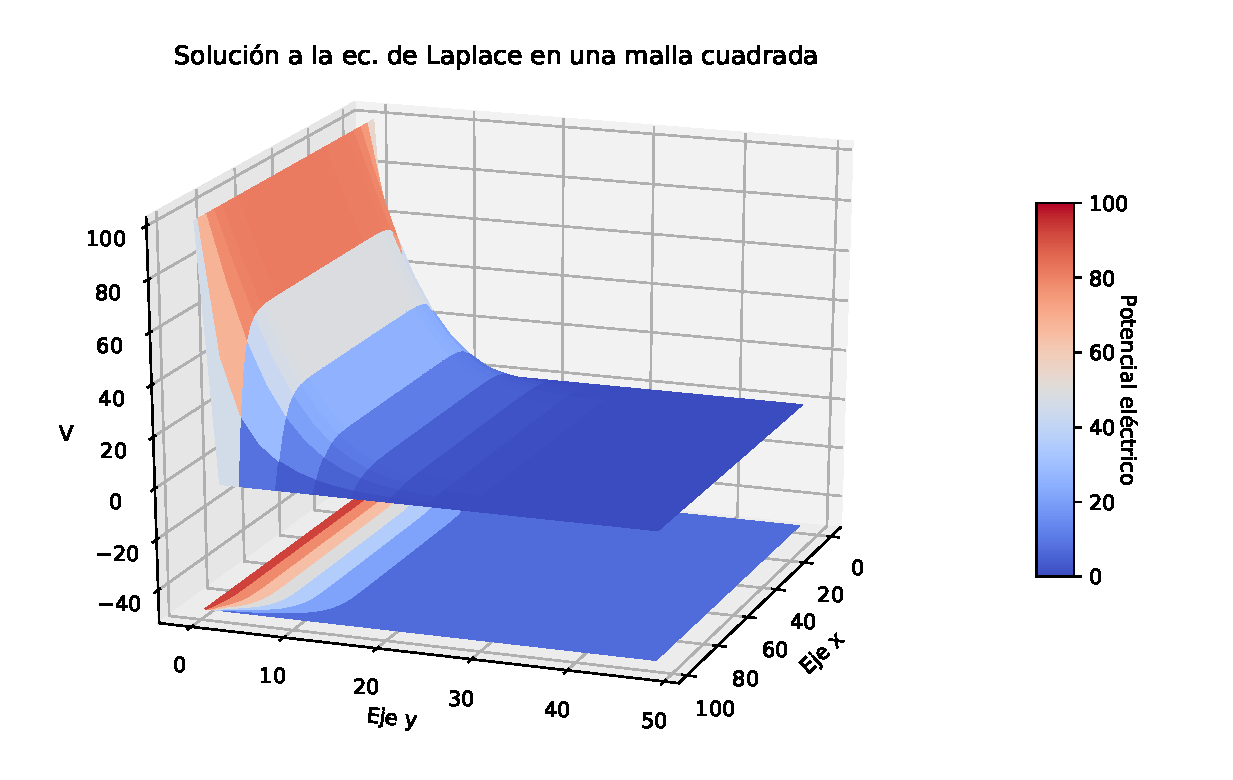
\includegraphics[scale=0.55]{Imagenes/ejercicio_Laplace_Potencial_01.eps} 
\end{figure}
\end{frame}
}
\begin{frame}
\frametitle{Sobre el proceso de solución}
Hemos visto un caso particular de la ec. de Laplace, con una geometría específica y con condiciones de frontera, también particulares.
\\
\bigskip
Con el esquema de trabajo de la presentación anterior, podemos resolver de la misma manera este ejercicio, ya que se planteó como un esquema general.
\end{frame}
\begin{frame}
\frametitle{Sobre el proceso de solución}
Si quisiéramos aplicar el esquema de este ejercicio a un caso más general, no podríamos utilizarlo.
\\
\bigskip
Es por ello que debemos de considerar varios aspectos para decidir, qué estrategia debemos escoger.
\end{frame}
\subsection{Ejercicios a cuenta}
\begin{frame}
\frametitle{Consideraciones}
Para cada uno de los ejercicios a cuenta, deberás de seguir el esquema de trabajo con la geometría cuadrada para la ecuación de Laplace.
\\
\bigskip
Revisa con cuidado cada punto en el enunciado del ejercicio, con ello, podrás realizar el respectivo código.
\end{frame}
\begin{frame}
\frametitle{1. Condensador de placas paralelas}
Ahora haremos un cambio en la geometría y dificultad del problema: vamos a considerar el caso de un condensador de placas paralelas, tal como se muestra en  la siguiente figura.
\end{frame}
\captionsetup[figure]{labelfont={color=blue}}
\begin{frame}
\frametitle{Geometría para el problema}
\begin{figure}
	\centering
	\includestandalone{Figuras/ejercicio_01_Tarea_Examen}
	\caption{Los valores de $w$ y de $d$ los estableces antes de proponer la solución, recuerda que cada barra mantiene el voltaje durante las iteraciones.}
\end{figure}
\end{frame}
\begin{frame}
\frametitle{Consideraciones}
Tienes que resolver la ecuación para calcular el potencial en cada punto, toma en cuenta lo siguiente:
\setbeamercolor{item projected}{bg=red!70!black,fg=white}
\setbeamertemplate{enumerate items}[circle]
\begin{enumerate}[<+->]
\item Usa un cuadro de $100 \cp 100$ para tener una mejor visualización.
\item Las líneas con potencial constante, tienen una longitud $w$, tal que $w < L$  (es decir, no van de un extremo al otro)
\seti
\end{enumerate}
\end{frame}
\begin{frame}
\frametitle{Consideraciones}
\setbeamercolor{item projected}{bg=red!70!black,fg=white}
\setbeamertemplate{enumerate items}[circle]
\begin{enumerate}[<+->]
\conti
\item Hay una separación $d$ que es constante entre las dos líneas de equipotencial.
\item Una vez con la solución de la EDP, grafica tus resultados.
\end{enumerate}
\pause
La siguiente gráfica corresponde a la solución.
\end{frame}
{\setbeamercolor{background canvas}{bg=white}
\begin{frame}[fragile]
\frametitle{Solución al problema de las placas}
\begin{figure}
	\centering
	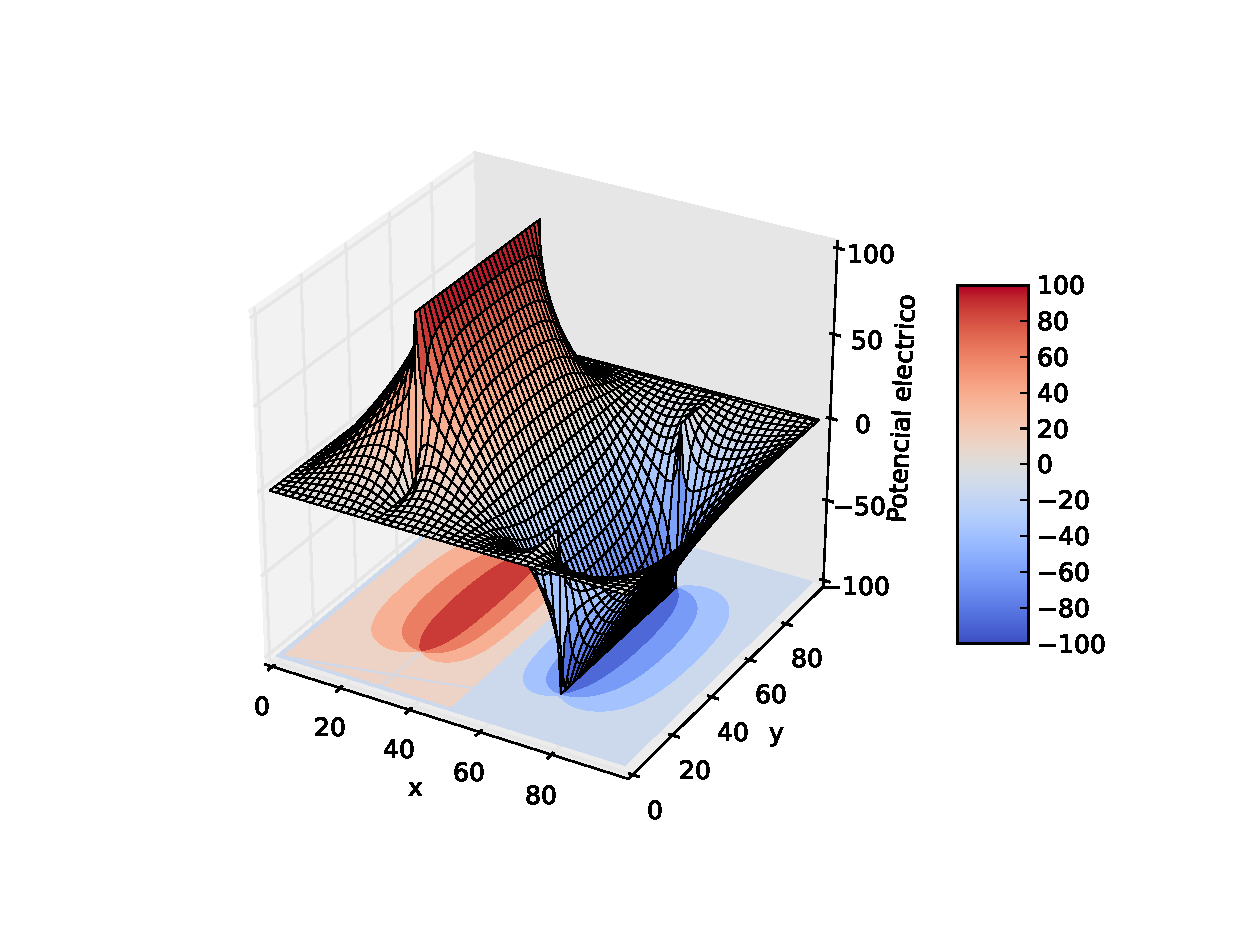
\includegraphics[scale=0.45]{Potencial02.eps} 
\end{figure}
\end{frame}
}
\begin{frame}
\frametitle{2. Placa cuadrada con potencial}
Resuelve la ecuación de Laplace con el siguiente arreglo donde la placa cuadrada conductora se encuentra a $\SI{1}{\volt}$ (geométricamente se localiza en el centro de la placa exterior, por lo que deberás de determinar su tamaño) mientras que la placa cuadrada exterior, se encuentra a $0$ volts.
\end{frame}
{\setbeamercolor{background canvas}{bg=white}
\begin{frame}
\frametitle{2. Problema a cuenta del examen}
\begin{figure}
	\centering
	\includestandalone[scale=0.9]{Figuras/ejercicio_02_Tarea_Examen}
	\caption{Las dimensiones de cada cuadrado las determinas nuevamente antes del iniciar la solución.}
\end{figure}
\end{frame}
}
%Referencia Beu. Problem 13.3
\begin{frame}
\frametitle{3. Placa cuadrada}
Considera una placa de metal cuadrada cuyos lados miden $L = \SI{10}{\centi\metre}$. La temperatura varía a lo largo de la frontera izquierda de acuerdo a $u(0, y) = 100 \, \sin (\pi \, y /L)$, mostrando un máximo en la mitad de la placa y anulándose en las esquinas y a los largo de los otros tres extremos.
\end{frame}
\begin{frame}
\frametitle{3. Placa cuadrada}
Determina el perfil de temperatura en la placa resolviendo la ecuación de calor:
\begin{align}
\pdv[2]{u}{x} + \pdv[2]{u}{y} = 0
\label{eq:ecuacion_13_147}
\end{align}
en el dominio $\mathcal{D} = [0, L] \cp [0, L]$ con las condiciones de contorno
\begin{align}
\begin{aligned}
u(0, y) &= 100 \, \sin (\pi \, y / L), \hspace{0.3cm} u(L, y) = 0, \hspace{0.2cm} y \in [0, L] \\[0.5em]
u(x, 0) &= u(x, L) = 0 \hspace{2cm} x \in [0, L]
\end{aligned}
\label{eq:ecuacion_13_148}
\end{align}
\end{frame}
\begin{frame}
\frametitle{Gráfica que debes de obtener}
\begin{figure}[h!]
    \centering
    \includegraphics[scale=0.35]{Imagenes/ejercicio_Laplace_Potencial_Placa_02.png}
    \caption{Solución al ejercicio}
\end{figure}
\end{frame}
\begin{frame}
\frametitle{De la gráfica obtenida}
La gráfica anterior muestra el contorno de temperaturas en la placa, no se muestra la superficie en $3D$, pero la puedes incluir, solo revisa bien tu código para que obtengas el contorno en $2D$.
\end{frame}
\end{document}